\chapter{水声传感网络MAC协议研究现状 }
\section{水声传感网络MAC协议分类}
\begin{figure}[ht]
	\centering
	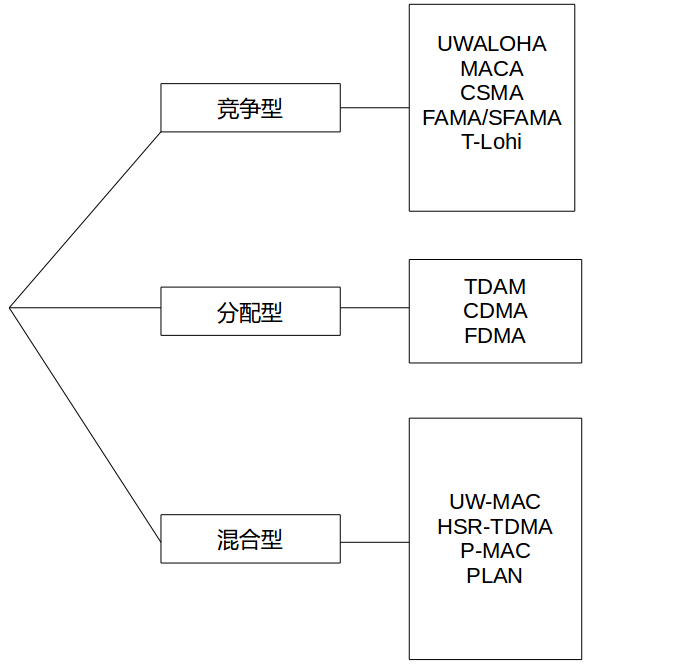
\includegraphics[scale=0.4]{figures/fenlei.png}
	\caption{
		MAC协议的分类和典型代表
	}
	\label{fig:example}
\end{figure}
MAC协议控制着信道的接入模式。如果不能有效得利用信道,不必要的冲突会导致整体网络性能的降低。因此设计MAC协议的基本目标应该是减少信道冲突。同时,MAC协议还需要考虑能量使用效率,网络可靠性和可扩展性等等因素。

两个或多个MAC帧同时到达同一接收节点就会产生冲突。传统的陆上MAC协议是通过时隙分配或者信道感知的方法来解决这种时间不确定性的。但由于水声信道的特殊性,水下MAC协议需要考虑的问题比之陆地环境更多更复杂。

传统的MAC协议分类方式在水下MAC协议中仍然是有效且实用的。MAC协议通过信道占用方法可以分为竞争协议、非竞争协议和混合协议。竞争协议包括了ALOHA、载波侦听多址接入CSMA、基站捕获多址接入FAMA、冲突避免多址接入MACA等;非竞争协议包括了时分多址TDMA、时空MAC、码分多址CDMA、频分多址FDMA;混合协议包括了综合TDMA和CDMA的混合空间
复用HSR-TDMAC,CDMA和ALOHA结合的UW-MAC等。
\subsection{竞争协议}
ALOHA协议是最早被提出应用于媒体接入控制的竞争性协议。它不进行预先的信道检测,在有数据包发送时就直接发送。ALOHA协议在网络负载较高时容易因频繁的数据冲突造成吞吐量下降。

在时隙ALOHA协议(Alotted ALOHA)中,节点在固定时隙的开始时刻进行传输,这种方法有效降低了数据的冲突,提高了网络吞吐量。基于载波侦听的ALOHA(ALOHA-CS)\cite{chirdchoo2007aloha},为了避免与正在进行的传输冲突,在发送数据包前会监测信道状态,在信道空闲状态下再进行传输。基于冲突避免的ALOHA(ALOHA-CA)\cite{chirdchoo2007aloha},通过接收信道中正在传输的包和记录网络中所有节点间的传播时延来避免冲突。基于预先提醒的ALOHA(ALOHA-AN)\cite{chirdchoo2007aloha},会在发送数据包前发送一个包括收发节点信息的短包来预约信道。

载波侦听多址接入(Carrier Sense Multiple Access, CSMA)在发送数据前会先侦听信道状态,当信道空闲时才发送数据,从而降低数据包冲突的概率。和aloha-CS不同,CSMA在侦听到信道空闲后并不立即发送,而是会进行随机退避来减小数据包碰撞概率。在p-坚持CSMA中,侦听到信道空闲后,节点以概率p进行传送,以1-p的概率进行退避。1-坚持 CSMA就等同于aloha-CS。但是,在长传播时延的水声传感网络中,信道侦听的效果有限,无法解决多跳网络的隐藏终端和暴露终端问题。

最初的基站捕获多址接入(Floor Acquisition Multiple Access,FAMA)需要长RTS和CTS帧来避免数据包传输的冲突。但是,在水声信道中,一次传输的开销很大,过长的控制帧同时也会带来很大的能量损耗。因此,为了减少控制帧的长度,提出了时隙FAMA(slotted FAMA)\cite{molins2007slotted}协议。时隙的长度等于最大传播时延加上一次控制帧传输时间。SFAMA是用控制帧的竞争代替了数据帧的竞争。

水声MACA\cite{ng2008maca}协议是在MACA协议基础上改进的竞争式水声MAC协议。MACA协议应用了RTS/CTS机制。通过发送RTS包预约信道,同时使邻居节点退避。通过CTS包可以通知目标节点的邻居节点进行退避。水声MACA协议考虑了节点转发数据需求,设定节点转发数据的优先级高于发送数据,因为待转发数据之前已经过一次或者多次传输,已经使用了网络资源,如果丢弃将带来更多的浪费。同时,协议在算法上对控制包握手交互过程进行了简单改进,主要是在三种情况下(分别为等待CTS时收到其他节点的RTS,等待DATA时收到其他节点的RTS和等待DATA时收到其他节点的CTS),将原来协议的进入安静状态改为不做任何操作。如果在安静状态接收到其他节点的RTS或者CTS,则通过计算继续保持安静状态到较大的时间值。这种改变有助于降低延时,提高吞吐量。但该协议会因为节点进入安静状态,造成其前跳节点不知道其具体情况而多次发送RTS请求,造成资源和能量的浪费。

T-Lohi\cite{syed2008t}的应用场景是单跳水声通信网络。T-Lohi协议将数据交互过程分为竞争阶段和数据传输阶段。协议中每个节点在每次发送数据前,先发送一个试探网络状况的短控制包(tone)。发送完tone数据后侦听网络中其它节点的tone数据,通过网络中tone的个数,判断整个网络繁忙程度。若有多个tone同时存在于信道中,则退避一定时间后再进行信道竞争,直到信道中只有一个tone,表明该节点成功竞争到信遒。在数据传输阶段发送数据。T-Lohi协议在传输数据时且简化了握手和消除冲突的机制,但是需要保证网络中的节点可侦听到整个网络的数据,因此不能解决在多跳网络环境中的隐藏终端暴露终端的问题。

\subsection{非竞争协议}
频分多址(Frequency Division Multiple Access, FDMA)把信道分为多个子信道,然后将子信道分配给不同的节点使用,允许不同节点在同一时刻无冲突的收发数据。虽然FDMA在陆地无线网络的性能很好,但由于水声信道的可用带宽窄,传输信道的相干带宽可能大于子信道的带宽。FDMA在应对衰减和多径问题上表现也很差。特别是,如果在数据量大的水声传感器网络中,由于子信道是固定分配给节点的,不具有适应动态变化的网络环境的能力,因此FDMA的性能较差。

时分多路复用(Time Division Multiple Access, TDMA)是把时间划分为时间间隙后分给节点的接入方法,每个节点只在给定的间隙传送数据。但是,TDMA为了避免节点之间分配的时间间隙有冲突,需要在每个间隙后加入一个保护时间,开销大。并且水下环境的长传输时延使得TDMA时间同步很难实现,因此会发生数据冲突,降低系统性能。

时空MAC将TDMA协议的分配问题看成定点着色问题。构建一个时空冲突图描述传输链路之间的冲突时延。然后根据混合整数线性规划模型求解出最优解,根据求解出的最优解进行时隙分配。

码分多址复用(Code Division Mmtiple Access, CDMA)允许所有节点同时在同一个信道上发送数据,它是通过给每个节点分配不同的扩频码来完成的。这些扩频码相互正交。和FDMA相比,CDMA不需要考虑信道对不同频率的选择性衰减。和TDMA相比它提高了对时间的利用率。缺点是相互正交的扩频码意味着要传输的编码长度很长,通信速率不高。

\subsection{混合协议}
在混合空间复用协议(Hybrid Spatial Reuse TDMA, HSR-TDMA)\cite{diamant2011spatial}中,由于水声传感网络的节点较少,各节点之间的邻近节点不是很多,因此对邻近节点分配了正交的扩频码后,这样网络中各节点可与其邻近节点同时进行通信,在多跳水声传感网络中,时隙还可以进行空间复用提高信道利用率。

UW-MAC\cite{watfa2010uw}考虑到网络各节点固定分配扩频码时需要较长的码长,对各节点的扩频码进行动态分配,只对当前要进行通信的节点进行分配扩频码,使得扩频码长得到了很大的降低,提高了网络信道利用率。

\section{移动水声传感网络MAC协议研究现状}
根据移动水声网络的分布式特性和可扩展性,Francisco Salvá-Garau和Milica Stojanovic提出了多集群协议(Multi-Cluster MAC)\cite{salva2003multi}。邻近节点分在一个集群中,在单个集群内使用统一的TDMA协议通信,不同集群间通过分配不同的扩频码来减少串扰、提高扩展性。协议分为两个阶段,首先在初始化阶段分配不同集群,然后进入持续时间较长的稳定传输阶段。

考虑到移动水声网络的低速率特性,Youngtae Noh和Uichin Lee等在2014年提出了DOTS(A Propagation Delay-Aware Opportunistic MAC Protocol for Mobile Underwater Networks)协议。节点通过被动获得的本地信息,如邻居节点传播时延表以及预期调度时序等,实现同一信道上多数据包并行发送。\cite{noh2014dots}

对于有移动节点接入的小规模单跳传感网络,毛佳、徐元欣等提出了LTM-MAC(Location-based TDMA MAC protocol for mobile underwater networks)\cite{mao2016ltm},协议给移动节点的接入分配了较高的优先级。对于移动节点接入的小规模多跳传感网络,他们提出了TMM-MAC协议(TDMA-based MAC for Multiple-hops in mobile underwater networks)。协议利用多跳特性,允许与移动节点互不干扰的固定节点并行发送数据,同时根据数据包长短设计不同的发送机制。

基于移动节点进行数据收集的情景,邓敏、陈惠芳等人提出了混合MAC协议\cite{deng2017hybrid},在低负载的子网中采用基于竞争的CT-MAC(ConTention-based MAC),在高负载的子网中采用基于轮询调度的RSV-MAC(ReSerVation-based MAC)。



\endinput